% !TeX root = ../rapport.tex
\chapter{Indledning}

\section{Problemformulering}
At designe og fremstille et éndimensionelt vognmonteret omvendt pendul, der ved hjælp af regulering skal kunne fastholde en forudbestemt vinkel af pendulet, samt at kunne kompensere for udefrakommende påvirkninger. 

\subsection{Formål}

\subsection{Krav til rapporten stillet i projektoplæg}
Måling og generering af elektromagnetiske felter kombineret med analog signalbehandling.
\husk{JJ}{Husk at opdatere projektoplægs krav inkl. ref. til oplæg}
\begin{itemize}
\item E-EEP (Elektromagnetisme, Elektronik og Projekt).
\item E-RMK (Regulering, Matematik og Kredsløbsteknik).
\end{itemize}

\subsection{Selvvalgte krav til produktet} \label{afs:kravspecifikation}
\begin{itemize}
\item Systemet skal kunne opretholde en maksimal svingvinkel af pendulet på 20 grader.
\item (Masser af systemet)
\item Systemet skal kunne drives af et/to batteri(er)
\item Sensoren skal være induktiv
\end{itemize}

\subsection{Problemstilling}
Følgende problemstillinger ønskes besvaret:
\begin{itemize}
\item Første
\item Anden
\end{itemize}

\subsection{Projektafgrænsning}
Følgende medtages ikke i rapporten og afgrænser projektarbejdet:
\begin{itemize}
\item Systemet skal kun virke i én retning (dimension)
\item Der ses bort fra fysisk beskrivelse af elektromotoren.
\item Der ses bort fra beskrivelsen af motorstyringen.
\item Vogn samt tilhørende motor, hjul og gearing overtages fra tidligere projekt.
\end{itemize}

\section{Løsningsmodel}
Blokdiagrammet her ?
\husk{JJ}{Del diagram af system og signalvej ?}

\section{Læsevejledning}
Rapportens læsevejledning...\\
Naturlig indførelse i emnet

\section{Arbejdsmetode}
Noter til arbejdsmetoden.
\begin{itemize}
	\item Iterativ planlægning
	\item ugentlige status møder hvor der opsummeres
	\item fleksibel opgave styring, for maksimal udnyttelse af ressourcer 
	\item To-Do lister
\end{itemize}

\section{Blokdiagram}
\begin{figure}[h!]
	\centering
	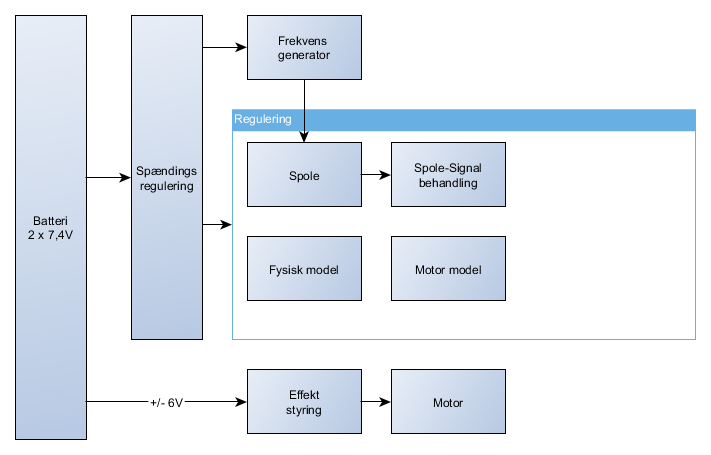
\includegraphics[width=.9\textwidth]{diagram/blokdiagram1.png}
	\caption{System blokdiagram.}
	\label{fig:blockdiagram1}
\end{figure}
\FloatBlock




